\documentclass[10pt,a4paper]{article}
\usepackage[utf8]{inputenc}
\usepackage[czech]{babel}
\usepackage[T1]{fontenc}

\usepackage{verbatim}
\usepackage{listings}
\usepackage{color}
\usepackage{xcolor}
\usepackage{textcomp}
\usepackage{url}
\usepackage{graphicx}

\definecolor{mygreen}{rgb}{0,0.6,0}
\definecolor{mygray}{rgb}{0.5,0.5,0.5}
\definecolor{mymauve}{rgb}{0.58,0,0.82}

\lstdefinestyle{sources}
{%
	backgroundcolor=\color{white},   % Pozadí
	commentstyle=\color{mygreen},    % Komentáře
	keywordstyle=\color{blue},       % Klíčová slova jazyka
	stringstyle=\color{mymauve},     % Řetězce
}

\lstset
{%
	%
	% Základní nastavení
	%
	basicstyle=\footnotesize,        % Styl a typ písma
	captionpos=b,                    % Pozice popisku
	showstringspaces=false,          % Když true, místo mezer se vypíše podtržítko. e.g. "Hello_world"
	title=\lstname,                  % Při výpisu zdrojového kódu ze souboru, nastaví název souboru jako popisek
	tabsize=4,                       % Velikost tabulátoru (počet mezer)
	style=sources,
	%
	% Podpora českých znaků
	% http://tex.stackexchange.com/questions/30512/how-to-insert-code-with-accents-with-listings/85947#85947
	%
	literate=
		{á}{{\'a}}1     {í}{{\'i}}1     {é}{{\'e}}1
		{ý}{{\'y}}1     {ú}{{\'u}}1     {ó}{{\'o}}1
		{ě}{{\v{e}}}1   {š}{{\v{s}}}1   {č}{{\v{c}}}1
		{ř}{{\v{r}}}1   {ž}{{\v{z}}}1   {ď}{{\v{d}}}1
		{ť}{{\v{t}}}1   {ň}{{\v{n}}}1   {ů}{{\r{u}}}1
		{Á}{{\'A}}1     {Í}{{\'I}}1     {É}{{\'E}}1
		{Ý}{{\'Y}}1     {Ú}{{\'U}}1     {Ó}{{\'O}}1
		{Ě}{{\v{E}}}1   {Š}{{\v{S}}}1   {Č}{{\v{C}}}1
		{Ř}{{\v{R}}}1   {Ž}{{\v{Z}}}1   {Ď}{{\v{D}}}1
		{Ť}{{\v{T}}}1   {Ň}{{\v{N}}}1   {Ů}{{\r{U}}}1
	,
}

\title{Determine applications affected by upgrade}
\author{Jakub Kadlčík}

\begin{document}
	% Vazba
	\maketitle
	\newpage

	% Anotace

	% Poděkování

	\tableofcontents
	\newpage

	\section{Úvod}
		\subsection{Správa software v GNU/Linux}
		Ve většině distribucí GNU/Linuxu se software standardně spravuje prostřednictvím balíčkovacího systému. Nové distribuce většinou vznikají odvozením jiné, již existující distribuce a v tomto případě bývá zachován typ balíčků i balíčkovací systém. Můžeme tedy říct, že distribucí je mnoho, ale balíčkovaích systémů se používá jen velmi málo. Konkrétně lze hovořit o distribucích GNU/Linuxu používající balíčky RPM\footnote{RPM = Red Hat Package Manager}, DEB\footnote{DEB = Debian software package} a nebo jiný typ balíčku. V posledním případě se jedná případ od případu o velmi specifický předpis balíčku. V rámci této práce se budeme zabývat linuxovou distribucí Fedora jako reprezentantem první skupiny a distribucí Gentoo, jako reprezentantem poslední skupiny.

			\subsubsection{Balíčkovací systém distribuce Fedora}
			Fedora vznikla jako nekomerční odnož Red Hat Linuxu a zachovala stávající systém balíčků RPM\@. Od své první verze využívá nástavbu nad RPM zvanou YUM\@. Ten se po čase stal téměř neudržovatelný a proto se objevila alternativa pojmenovaná DNF\@. V současné době lze paralelně využívat oba tyto nástroje, avšak je snaha YUM kompletně nahradit za pomocí DNF\@. Mělo by k tomu dojít již ve Fedoře 21. Aktuální stabilní verze je 20, jde tedy o příští vydání.

			\subsubsection{Balíčkovací systém distribuce Gentoo}

		\subsection{Problém}
		Když spustíme aplikaci, do paměti se načtou knihovny a soubory potřebné k jejímu běhu. Pokud je některá z knihoven, nebo samotná aplikace po dobu jejího běhu aktualizována, v paměti stále zůstanou původní soubory, přestože fyzicky už nemusí existovat (mohou být smazány, nebo nahrazeny novějšími verzemi).
		\\\\
		Zjistit, které, v systému spuštěné, aplikace využívají takto neaktuální soubory, není pro uživatele triviální. V současné době sice existují nástroje, které tento problém řeší, avšak jsou z mnoha důvodů nedostatečné.

		\subsection{Motivace}
		Na první pohled by se mohlo zdát, že postrádá smysl, zabývat se takovým problémem a jeho vyřešení nepřinese nic zajímavého. Ve skutečnosti však mohou být důsledky velmi nebezpečné. Pokud například aktualizace opravuje bezpečnostní chybu staré verze, běžící aplikace zůstanou neopravené. K jejich opravě dojde až jejich restartováním. Uživateli se tak může stát, že nainstaluje záplatu, bude si myslet, že jeho systém je opět bezpečný a přitom stále běží několik nebezpečných procesů.
		\\
		Další problém se týká spíše uživatelů \textit{unstable} distribucí, kterým do systému mohou přicházet zpětně nekompatibilní balíčky. Potom se může stát, že některá služba odmítne nastartovat, protože nová verze nepovoluje stávající konfiguraci, nebo vlivem nepřesně specifikovaných závislostí zůstane v systému nekompatibilní verze knihovny. Takovýchto případů bychom si rádi všimli co nejdříve to bude možné, nikoliv až v kritické chvíli, kdy například dojde k restartování serveru.

		\subsection{Požadavky}
		Tato práce si klade za cíl vytvořit software, který bude řešit problém \textit{nalezení aktualizacemi ovlivněných aplikací}. Software by měl najít všechny programy využívající neaktuální soubory a doporučit jejich restartování. Pro různé typy programů by měla být vypsána jiná doporučení a nápověda, jakým způsobem to lze provést. Software by měl disponovat textovým uživatelským rozhraním a mělo by být možné jej používat jako modul přímo v balíčkovacím systému DNF\@. Vývoj by měl probíhat pod otevřenou licencí a na libovolném veřejném úložišti. Dále by měl být k dispozici instalační balíček pro distribuci Fedora.

	\section{Analýza}
	Rozložme si problém na menší části a projděme je jednu po druhé. Stěžení funkcí má být vypsání jistého seznamu aplikací. Nejdříve se tedy zaměříme na jeho získání. Dále potřebujeme konstrukt, který zjistí informace o  dané aplikaci. Nakonec se budeme zajímat o to, jakým způsobem lze nalezené aplikace restartovat.

		\subsection{Seznam ovlivněných aplikací -- Ilustrativně}
		Stěžejní funkcí bude nalezení aktualizacemi ovlivněných, běžících aplikací. Řešení se zdá být velmi přímočaré. Nejdříve zjistit seznam balíčků, které byly od spuštění systému modifikovány. Následně pro každý balíček zjistit seznam souborů, které poskytuje. Poté zjistit, které procesy využívají některý z množiny modifikovaných souborů. Tedy pro každý spuštěný proces zjistit seznam souborů jež využívá a najít shodu se soubory poskytovanými modifikovanými balíčky.

		\lstinputlisting
		[
			language={Python},
			label=naive-tracer-algorithm,
			caption={Algoritmus pro vypsání seznamu ovlivněných aplikací}
		]{sources/naive_tracer_algorithm.py}

		Algoritmus na první pohled vypadá velmi jednoduše a zřejmě vypíše korektní množinu procesů. Mohlo by se tedy zdát, že máme hotovo, nicméně jsme nevzali v úvahu časovou složitost takového algoritmu. Ta, jak si ukážeme níže, je bohužel velmi nepříznivá, což by vedlo k útrpně pomalému vyhledávání.

			\subsubsection*{Časová složitost}
			Časovou složitost lze vyjádřit následovně. První průchod přes všechny balíky je lineární, tedy $O(n)$. Pro každý balík se prochází všemi procesy, takže násobíme $* O(m)$. Protože jsou obě $m$ i $n$ spočetně velké a nejsou to konstanty, místo $O(n*m)$ vyjádříme $O(n^2)$.
			\\
			\\
			Dále počítáme složitost množinového průniku. V případě jeho naivní implementace, která porovnává každý prvek jedné množiny s každým prvkem druhé, dostaneme kvadratickou složitost $O(n^2)$. V případě optimalizovanějšího návrhu si polepšíme na $O(n)$.
			\\
			\\
			Množinový průnik je zjišťován pro každou kombinaci balíčku a procesu, proto původní $O(n^2)$ násobíme $O(n)$ (případně $O(n^2)$ při naivní implementaci). Výslednou časovou složitost ukázaného algoritmu tedy vyčíslíme jako $O(n^3)$.

			% Úvaha, zda to půjde lépe + graf

			\subsubsection*{Existuje způsob, jak to udělat lépe?}
			Nyní se dostáváme do situace, kdy si musíme položit následující otázku -- Existuje vůbec způsob, jak to udělat lépe?
			\\
			\\
			@TODO Dopsat po kurzu Vyčíslitelnost a složitost.\\
			@FIXME Na kurzu Vyčíslitelnost a složitost jsem asi nedával dostatečně pozor

		\subsection{Seznam ovlivněných aplikací -- Vylepšení}
		Klíčem k rychlejšímu získání chtěných procesů je zvolení vhodné vyhledávací struktury pro data. Vezměme si fakt, že mnoho procesů využívá stejné soubory (knihovny, etc). Naivní algoritmus tedy jeden konkrétní soubor musí ověřit hned několikrát -- pro každý proces, který jej využívá.

		Tento nedostatek můžeme řešit tak, že nebudueme zkoumat proces po procesu, ale místo toho vezmeme množinu všech\footnote{} souborů v paměti, přičemž ke každému souboru si poznačíme procesy, které jej využívají. Pro nejrychlejší možné vyhledávání v množině souborů, zvolíme strom typu BTree jako strukturu pro uložení dat. Zaplatíme sice zvýšenou spotřebou paměti, ale jak si ukážeme v kapitole XY, rychlostní zlepšení bude na první pohled zjevné.

		\lstinputlisting
		[
			language={Python},
			label=tracer-algorithm,
			caption={Vylepšený algoritmus pro vypsání seznamu ovlivněných aplikací}
		]{sources/tracer_algorithm.py}

			\subsubsection*{Časová složitost}
			Při vyhledávání je pro každý balíček v seznamu procházen seznam jím poskytovaných souborů. Složitost tohoto problému je analogická předchozí situaci -- Tedy $O(n^2)$. Co se ovšem změnilo, je problém nalezení všech procesů, využívajících daný soubor. Nyní si stačí vyzvednout jejich seznam jednorázovým přístupem do stromové struktury typu BTree. Složitost tohoto problému je $O(log(n)$. Poskládáním jednotlivých kousků problému dohromady, získáváme časové složitost algoritmu vyjádřenou jako $O(n^2 * log(n))$.

		\subsection{Informace o aplikaci}
		Rozlišujme dva druhy informací. Pracujeme se spuštěnými aplikacemi, tedy lze hovořit o procesech spuštěných v systému. Každý proces má nějaký PID\footnote{}, spustil jej nějaký uživatel, běží určitou dobu, etc.

		Dále lze uvažovat, že každá\footnote{Každá standardně nainstalovaná} aplikace je poskytována distribučním balíčkem. Každý takový balíček poskytuje informace o tom, k čemu slouží, v jaké je verzi, jak dlouho je nainstalován, etc.

		Lze předpokládat, že informace o procesech budou získatelné jednotným způsobem napříč celým spektrem linuxových distribucí, avšak informace o balíčku budou závislé na jeho typu.

		\subsection{Jak aplikaci restartovat?}
		Aplikace můžeme rozdělit do několika kategorií. Zřejmě budou existovat takové, jež nemůžeme restartovat jinak, než rebootováním celého operačního systému. Příkladem budiž init, či jaderné procesy. Dále jistě budou v systémech s grafickým uživatelským rozhraním aplikace, k jejichž restartování bude potřeba řestartovat celé grafické prostředí. Příkladem mohou být správci oken a aplikace související s uživatelským sezením\footnote{Známnějsí spíše v anglickém originale jako session}. V těchto případech nezbývá jiná možnost, než provést požadovanou operaci jako reboot počítače, či odhlášení a opětovné přihlášení uživatele do grafického režimu.
		\\
		\\
		Zajímavější situace je v případě aplikací, které lze restartovat pomocí příkazu v příkazové řádce. Ta je typická pro tzv.\ daemony, či služby. Napříč velkým spektrem distribucí a správců služeb, lze k jejich restartování standardně použít příkaz \texttt{service} \textit{název\_služby} \texttt{restart}. Využití u daemonů není výhradní, protože lze tímto způsobem přistupovat i ke spoustě běžných aplikací. U nich se ale budou jednotlivé příkazy fundamentálně lišit.
		\\
		\\
		Všechy ostatní aplikace spadají do poslední skupiny. Uživatel je musí ručně ukončit a znovu spustit. Nezáleží na tom, zda jsou grafické a bude tak učiněno křížkem v záhlaví okna, nebo spuštěné v příkazové řádce a budou ukončeny jiným způsobem. Tato poslední kategorie není bezpečně automatizovatelná a proto musí zůstat v plné režii uživatele.


	\pagebreak
	\section{Implementace}
		\subsection{Úvod}
		Projekt je vyvíjen pod názvem tracer. Požadovalo se, aby byl implementován v jazyce Python. V současné době se nejčastěji používá Python2.7, který lze nalézt na všech distribucích a pro který existuje velká spousta uživatelských knihoven. Z tohoto důvodu jsem zvolil právě verzi 2.7, přestože aktuální stabilní verzí je 3.x.

		\subsection{Práce s procesy}
		Správu procesů v jazyce python zajišťuje balík psutil, který je ve Fedoře k dispozici pod názvem python-psutil. Umožňuje přístup ke všem atributům procesu, které lze v linuxových systémech zjistit. Mimo to poskytuje rozhraní pro získávání informací o paměti, procesoru, pevných discích a síťových rozhraních.

		Nás ovšem zajímá pouze práce s procesy.

		\lstinputlisting
		[
			language={Python},
			label=psutil,
			caption={Základní práce s procesy v psutil}
		]{sources/psutil.py}

		Pokročilejší funkcí může být zjištění souborů, které proces využívá.

		\lstinputlisting
		[
			language={Python},
			label=process-files,
			caption={Výpis všech souborů, které proces využívá}
		]{sources/process_files.py}

		Výpis tohoto ukázkového kódů může vypadat následovně:

		\lstinputlisting
		[
			label=process-files-output,
			caption={Ukázka výstupu předchozího kódu}
		]{sources/process_files_output}

		\subsubsection{Problémy při práci s procesy}
		% @TODO Dopsat

		\subsection{Práce s balíčky}
			Především nás budou zajímat tři operace. Zjištění seznamu balíčků, které byly od daného času modifikovány, zjištění základních informací o balíčku jako například název, popis, etc a nakonec zjištění souborů, které balíček poskytuje. Ukážeme si, že každou z nich lze implementovat několika různými způsoby. Objasníme, který z nich bude vyhovovat nejvíce a proč.

			\subsubsection{Databáze balíčků}
			Úvodem uděláme drobnou odbočku a podíváme se, jakým způsobem jsou v systému reprezentovány informace o balíčcích.
			\\
			\\
			Balíčkovacím systémem distribuce Fedora je program zvaný DNF\@, který pro uchovávání historie prováděných operací s balíčky, využívá sqlite databázi v adresáři \texttt{/var/lib/dnf/history}. Z ní se můžeme dozvědět informace o všech proběhlých transakcích. Scháma databáze vypadá následovně.

			% Obrázek databáze
			% @TODO Přegenerovat- chybějící tabulka pkgtups
			%\begin{figure}
				%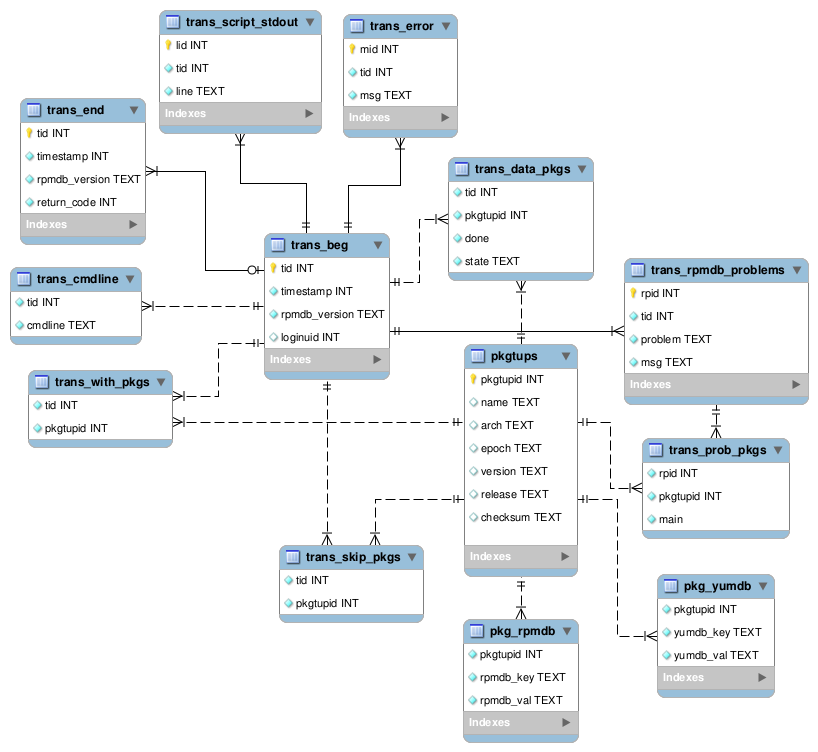
\includegraphics[scale=0.7]{images/dnf-database.png}
			%\end{figure}
			\centerline{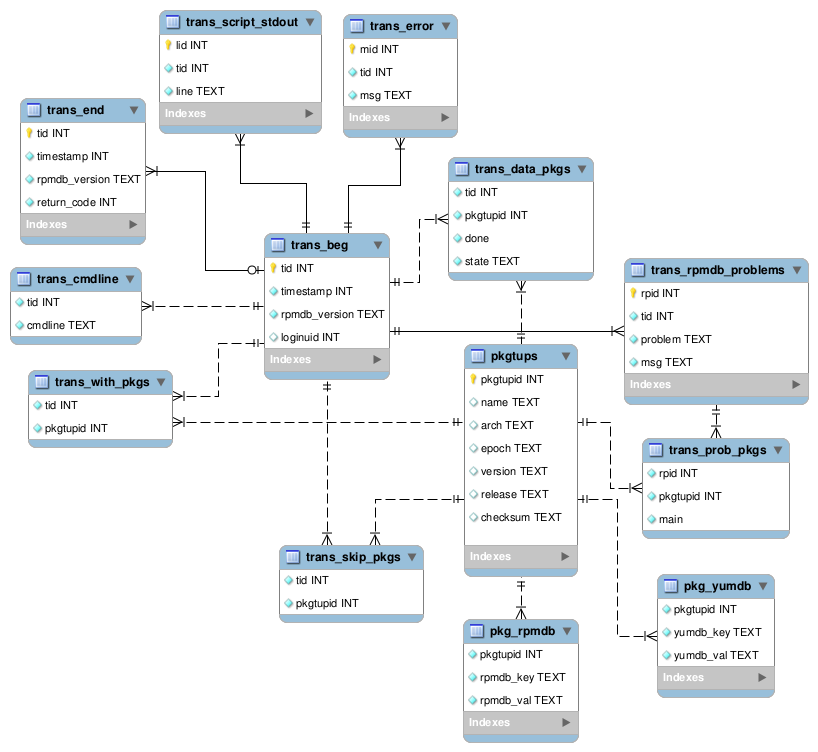
\includegraphics[scale=0.7]{images/dnf-database.png}}

			My se budeme zajímat výhradně úspěšně proběhlými transakcemi, proto nás tabulky, zabývající se chybami, nebudou zajímat. Nám užitečné informace se nacházejí především v tabulkách \texttt{trans\_beg}, \texttt{trans\_end}, \texttt{trans\_data\_pkgs} a \texttt{pkgtups}. Z prvních dvou lze zjistit, kdy byly spuštěny a dokončeny spuštěné transakce. Kterých balíčků se týkali a jaké operace s nimi byly prováděny popisuje tabulka \texttt{trans\_data\_pkgs}. Dané balíčky ovšem rozlišuje pouze pomocí jejich unikátního identifikátoru \texttt{pkgtupid}. K zjištění více informací o daném balíčku si jej musíme vyhledat v poslední zmíněné tabulce \texttt{pkgtups}.

			\subsubsection{Historie balíčků}
			Na základě znalostí z předchozí kapitoly můžeme bez dalších odboček přejít přímo ke zkoumání historie balíčků. V programovacím jazyce Python máme pro práci se sqlite databázemi k dispozici balíček \texttt{sqlite3}. Ten umožní dotazování se vůči databázi pomocí vlastních SQL dotazů. Nejdříve se tedy zaměříme na vytvoření dotazu pro získání všech balíčků modifikovaných od určitého bodu v čase.
			\\
			\\
			Informace o balíčcích, jako například jeho název, nebo verze, jsou uloženy v tabulce \texttt{pkgtups}. Není zde však datum jeho změny, proto musíme začít z druhého konce. Provedené transakce včetně času jejich spuštění se nacházejí v tabulce \texttt{trans\_beg}. Odtud dovedeme transakce spojit s relacemi v tabulce \texttt{trans\_data\_pkgs} přes atribut \texttt{tid}. Výsledkem spojení budou relace obsahující atribut \texttt{pkgtupid}, pomocí jenž můžeme provést spojení s tabulkou \texttt{pkgtups}, o kterou nám z počátku šlo.
			\\
			Současným mezivýsledkem jsou všechny relace vzniklé spojením zmíněných tabulek. Pomocí restrikce tuto relaci omezíme pouze na relace pro které platí, že atribut \texttt{trans\_beg.timestamp} nabývá hodnot větších, než $t$, kde $t$ je argument ve formátu zvaném jako Unix time\footnote{Známém také jako POSIX time, nebo Epoch time. Tento formát popisuje počet sekund uplynulých od 00:00:00 světového času dne 1.~1.~1970}.

			V jazyce SQL lze tento problém vyjádřit následovně.

			\lstinputlisting
			[
				language=SQL,
				label=packages-newer-than-sql,
				caption={Balíčky změněné od času $t$ - SQL dotaz}
			]{sources/packages_newer_than.sql}

			Pokračujme spuštěním tohoto dotazu v jazyce Python a získáním jeho výsledku. Předpokládejme předchozí dotaz uložený v proměnné \texttt{sql}, umístění databázového souboru v proměnné \texttt{db\_file} a libovolný čas v proměnné \texttt{unix\_time}. Tento zdrojový kód ukazuje, jak se lze dotázat vůči dané sqlite databázi a získat výsledek.

			\lstinputlisting
			[
				language=Python,
				label=packages-newer-than-py,
				caption={Balíčky změněné od času $t$ - Python}
			]{sources/packages_newer_than.py}

			Ukázkový kód je natolik sebevysvetlující, že se obejde bez většího komentáře. Za pozornost stojí především metoda \texttt{fetchall()}, která vrací seznam všech řádků výsledku. Ve výchozím nastavení jsou jednotlivé řádky reprezentovány datovou strukturou \texttt{tuple}. Jedná se o strukturu, která by se dala popsat jako uspořádaná n-tice. Při přístupu k hodnotám atributů potom záleží na jejich pořadí v n-tici. Tento přístup má velké nevýhody, proto na třetím řádku specifikujeme, že bychom chtěli jednotlivé řádky vracet reprezentované pomocí objektů třídy \texttt{sqlite3.Row}. To umožní přístup k atributům pomocí jejich názvů.

			\pagebreak
			\subsubsection{Informace o balíčku}
			Pro zjištění všech informací o balíčku můžeme použít příkaz

			% Pozor, balíček musí být nainstalován
			\begin{lstlisting}
				rpm -qi nazev_balicku
			\end{lstlisting}

			Výpis těch zajímavějších můžeme vidět zde
			\lstinputlisting
			[
				label=fedora-package-info-output,
				caption={Informace o balíčku}
			]{sources/fedora_package_info_output}

			Tyto informace můžeme v prostředí Pythonu získat a zpracovat v zásadě dvěma způsoby. Prvním je použití modulu \texttt{subprocess} ke spuštění výše zmíněného příkazu a získání jeho výstupu.
			\lstinputlisting
			[
				language=Python,
				label=fedora-package-info-parse,
				caption={Parsování informací o balíčku}
			]{sources/fedora_package_info_parse.py}

			Tato varianta však není ideální. Vyžaduje ruční parsování výtupu jakožto textového řetězce. Navíc dochází k drobnému zpomalení z důvodu spouštění nového procesu. Tato prodleva by byla zanedbatelná v případě jednorázového volání, ale zjišťování informací může být prováděno na větším množství balíčků, což by vedlo k výraznému zpomalení programu.

			Mnohem lepší variantou je použití aplikačního rozhraní poskytovaného modulem \texttt{rpm}, které nabídne čistějsí řešení, netrpící zmíněnými neduhy.

			\lstinputlisting
			[
				language=Python,
				label=fedora-package-info-api,
				caption={Získání informací o balíčku pomocí rpm API}
			]{sources/fedora_package_info_api.py}

			V tomto kódu se vyskytuje spousta neobjasněných elementů. Pojďme si je postupně projít a vysvětlit jejich význam. Každý skript pracující s balíčkem RPM musí zákonitě začínat instancováním třídy \texttt{TransactionSet}. Ta se postará o otevření databáze balíčků a poskytne rozhraní pro dotazování se vůči ní. Tím je metoda \texttt{dbMatch} použitá na následujícím řádku. Jejím výsledkem je vždy iterátor obsahující nalezené balíčky. To, jaké balíčky budou vráceny lze ovlivnit nastavením patřičných argumentů. V případě jejich vynechání, bude vrácen iterátor množiny všech nainstalovaných balíčků. Samozřejmě lze i vyhledávat pouze balíčky splňující určitá kritéria. V ukázkovém příkladu jsou vyhledány všechny balíčky, které se jmenují \texttt{vim-X11}. Jméno balíčku je však unikátní vlastnost, takže iterátor obsahuje pouze jednu položku (případně žádnou pokud nebyla nalezena shoda). Získáme ji pomocí metody \texttt{next()}.
			\\
			Jednotlivé balíčky jsou reprezentovány pomocí slovníků\footnote{Jiný název pro konstrukci známější především jako asociativní pole}. Jejich klíče jsou \texttt{"name"}, \texttt{"summary"}, \texttt{"group"} a tak podobně. Konstanty \texttt{RPMTAG\_SUMMARY}, \texttt{RPMTAG\_GROUP}, etc, jsou pouze tenká abstrakční vrstva vracející daný řetězec.

			\subsubsection{Seznam souborů poskytovaných balíčkem}
			Ke zjištění seznamu všech souborů, které daný balíček poskytuje, máme k dispozici příkaz

			% Pozor, balíček musí být nainstalován
			\begin{lstlisting}
				rpm -ql nazev_balicku
			\end{lstlisting}

			Pro získání a zpracování tohoto seznamu platí totéž co v předchozím případě. Varianta využívající modul \texttt{subprocess} by vypadala velmi podobně. Oproti předchozímu použití by se změnil pouze spouštěný příkaz. Navíc jsme tuto variantu implementace z dobrých důvodů vyloučili. Proto se budeme zabývat především použitím aplikačního rozhraní modulu \texttt{rpm}.

			% @TODO Popsat TransactionSet(), dbMatch(), next(), fi(), klíče f[]
			\lstinputlisting
			[
				language=Python,
				label=fedora-package-files-api,
				caption={Získání seznamu souborů poskyovaných balíčkem}
			]{sources/fedora_package_files_api.py}

		\subsection{Rozšíření pro balíčkovací systém DNF}
		\subsection{Tracer}
			V předchozích kapitolách jsme představili problematiku hledání aktualizacemi ovlivněných aplikací, popsali algoritmy pro jejich hledání a způsob, jak je lze implementovat v jazyce python pro linuxovou distribuci Fedora. Nyní se podíváme na produkt nesoucí název Tracer, jenž na těchto základech vznikl.
			\subsubsection{Uživatelská příručka}
				Následuje pouze nástin možných případů užití. Kompletní uživatelskou dokumentaci a manuálovou stránku programu naleznete v příloze XY.

				\paragraph{Standardní použití}
				Primárním a zároveň nejjednodušším způsobem, jak program spustit, je příkazem\footnote{Oprávnění superuživatele je nutné, protože program potřebuje číst databázi balíčkovacího systému.} \texttt{sudo tracer}. Na výstupu obdržíme seznam ovlivněných aplikací, tak jak byl požadován v zadání. Ukázkový výstup můžeme vidět na následujícím příkladu.

				% @TODO Aktualizovat výstup (i na docs.tracer-package.com)
				\lstinputlisting
				[
					label=tracer-standard-usage-output,
					caption={Ukázkový výstup příkazu \texttt{sudo tracer}}
				]{sources/tracer_standard_usage_output}

				\paragraph{Zobrazení konkrétní aplikace}
				Uživatel může ve výstupu narazit na aplikaci, kteoru například nezná, nebo netuší, proč a jak je potřeba ji restartovat. Z tohoto důvodu existuje přepínač \texttt{-s} neboli \texttt{--show}, který zobrazí všechny informace, které Tracer o aplikaci zná a se kterými pracuje.

				\lstinputlisting
				[
					label=tracer-helper-output,
					caption={Ukázkový výstup příkazu \texttt{sudo tracer -s apache2}}
				]{sources/tracer_helper_output}

				Stejně jako u většiny UNIXových programů, lze množství vypisovaných informací ovlivnit přepínači \texttt{-v} a \texttt{-vv}. První varianta zobrazí i seznam balíčků jenž aplikaci ovlivnil. Druhá varianta pak zobrazí i seznam konkrétních souborů, které balíčky aktualizovali a aplikace je využívá. Konečně, pro výpis těchto pomocných informací ke každé nalezené aplikaci lze zobrazit přepínačem \texttt{--helpers}.

				\paragraph{Interaktivní mód}
				V určitých případech může uživatel chtít zobrazit pomocné informace pouze k několika aplikacím, ale nechce vypisovat jejich názvy. Pro tento účel byl zaveden interaktivní režim. Pokud spustíme Tracer s parametrem \texttt{-i}, nebo \texttt{--interactive}, obdržíme na výstupu očíslovaný seznam aplikací zakončený promptem. Postupně zadáváme čísla aplikací, které nás zajímají a dostáváme výpis pomocných informací.

			\subsubsection{Adresářová struktura}
			\subsubsection{MVC}

		\subsection{DNF plugin}
		\subsection{Testování}

	\section{Distribuce programu}
		\subsection{Licence}
		\subsection{Zdrojový kód}
		\subsection{Verzování}
		\subsection{Balíčky pro distribuce}
		\subsection{Dokumentace}

	\section{Porovnání s konkurencí}
		\subsection{needs-restarting}
		\subsection{checkrestart}
		\subsection{needrestart}
		% https://github.com/liske/needrestart

	\section{Závěr} % Zrušit číslování
	\section{Conclusions} % Zrušit číslování
	\section{Reference} % Zrušit číslování

	% Obsah přiloženého CD
\end{document}
